\documentclass[12pt,a4paper]{article}
\usepackage{graphicx}
\title{Assignment - 4, Snell's law }
\author{Anan Madhav T V, MM22B013}
\date{18th june 2023}
\usepackage[letterpaper,top=2cm,bottom=2cm,left=3cm,right=3cm,marginparwidth=1.75cm]{geometry}


\begin{document}

\maketitle
\section{MM22B013}
Name : Anan Madhav T V\\
Github user-id : ananmadhav 

\subsection{Introduction}
Snell's law states that the relationship between the angles of incidence and refraction, when a light passes from one medium to another medium. Snell's law is also known as law of refraction.

\subsection{Statement of Snell's Law}

Snell's Law states that the ratio of the sine of the angle of incidence and the sine of the angle of refraction is always constant for a given pair of media.
\footnote{https://byjus.com/physics/law-refraction-snells-law/}

\begin{equation}
\frac{{\sin(i)}}{{\sin(r)}} = n 
\end{equation}

Here n refers to the ratio of refractive index of the medium r with respect to medium i.

\begin{center}
    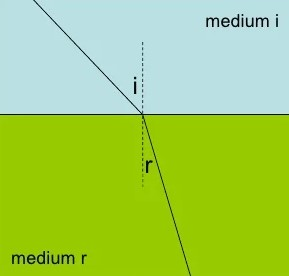
\includegraphics[width=0.5\textwidth]{snells law.jpg}    
\end{center}

\end{document}
